% Options for packages loaded elsewhere
\PassOptionsToPackage{unicode}{hyperref}
\PassOptionsToPackage{hyphens}{url}
%
\documentclass[
  oneside]{book}
\usepackage{amsmath,amssymb}
\usepackage{lmodern}
\usepackage{iftex}
\ifPDFTeX
  \usepackage[T1]{fontenc}
  \usepackage[utf8]{inputenc}
  \usepackage{textcomp} % provide euro and other symbols
\else % if luatex or xetex
  \usepackage{unicode-math}
  \defaultfontfeatures{Scale=MatchLowercase}
  \defaultfontfeatures[\rmfamily]{Ligatures=TeX,Scale=1}
\fi
% Use upquote if available, for straight quotes in verbatim environments
\IfFileExists{upquote.sty}{\usepackage{upquote}}{}
\IfFileExists{microtype.sty}{% use microtype if available
  \usepackage[]{microtype}
  \UseMicrotypeSet[protrusion]{basicmath} % disable protrusion for tt fonts
}{}
\makeatletter
\@ifundefined{KOMAClassName}{% if non-KOMA class
  \IfFileExists{parskip.sty}{%
    \usepackage{parskip}
  }{% else
    \setlength{\parindent}{0pt}
    \setlength{\parskip}{6pt plus 2pt minus 1pt}}
}{% if KOMA class
  \KOMAoptions{parskip=half}}
\makeatother
\usepackage{xcolor}
\usepackage{color}
\usepackage{fancyvrb}
\newcommand{\VerbBar}{|}
\newcommand{\VERB}{\Verb[commandchars=\\\{\}]}
\DefineVerbatimEnvironment{Highlighting}{Verbatim}{commandchars=\\\{\}}
% Add ',fontsize=\small' for more characters per line
\usepackage{framed}
\definecolor{shadecolor}{RGB}{248,248,248}
\newenvironment{Shaded}{\begin{snugshade}}{\end{snugshade}}
\newcommand{\AlertTok}[1]{\textcolor[rgb]{0.94,0.16,0.16}{#1}}
\newcommand{\AnnotationTok}[1]{\textcolor[rgb]{0.56,0.35,0.01}{\textbf{\textit{#1}}}}
\newcommand{\AttributeTok}[1]{\textcolor[rgb]{0.77,0.63,0.00}{#1}}
\newcommand{\BaseNTok}[1]{\textcolor[rgb]{0.00,0.00,0.81}{#1}}
\newcommand{\BuiltInTok}[1]{#1}
\newcommand{\CharTok}[1]{\textcolor[rgb]{0.31,0.60,0.02}{#1}}
\newcommand{\CommentTok}[1]{\textcolor[rgb]{0.56,0.35,0.01}{\textit{#1}}}
\newcommand{\CommentVarTok}[1]{\textcolor[rgb]{0.56,0.35,0.01}{\textbf{\textit{#1}}}}
\newcommand{\ConstantTok}[1]{\textcolor[rgb]{0.00,0.00,0.00}{#1}}
\newcommand{\ControlFlowTok}[1]{\textcolor[rgb]{0.13,0.29,0.53}{\textbf{#1}}}
\newcommand{\DataTypeTok}[1]{\textcolor[rgb]{0.13,0.29,0.53}{#1}}
\newcommand{\DecValTok}[1]{\textcolor[rgb]{0.00,0.00,0.81}{#1}}
\newcommand{\DocumentationTok}[1]{\textcolor[rgb]{0.56,0.35,0.01}{\textbf{\textit{#1}}}}
\newcommand{\ErrorTok}[1]{\textcolor[rgb]{0.64,0.00,0.00}{\textbf{#1}}}
\newcommand{\ExtensionTok}[1]{#1}
\newcommand{\FloatTok}[1]{\textcolor[rgb]{0.00,0.00,0.81}{#1}}
\newcommand{\FunctionTok}[1]{\textcolor[rgb]{0.00,0.00,0.00}{#1}}
\newcommand{\ImportTok}[1]{#1}
\newcommand{\InformationTok}[1]{\textcolor[rgb]{0.56,0.35,0.01}{\textbf{\textit{#1}}}}
\newcommand{\KeywordTok}[1]{\textcolor[rgb]{0.13,0.29,0.53}{\textbf{#1}}}
\newcommand{\NormalTok}[1]{#1}
\newcommand{\OperatorTok}[1]{\textcolor[rgb]{0.81,0.36,0.00}{\textbf{#1}}}
\newcommand{\OtherTok}[1]{\textcolor[rgb]{0.56,0.35,0.01}{#1}}
\newcommand{\PreprocessorTok}[1]{\textcolor[rgb]{0.56,0.35,0.01}{\textit{#1}}}
\newcommand{\RegionMarkerTok}[1]{#1}
\newcommand{\SpecialCharTok}[1]{\textcolor[rgb]{0.00,0.00,0.00}{#1}}
\newcommand{\SpecialStringTok}[1]{\textcolor[rgb]{0.31,0.60,0.02}{#1}}
\newcommand{\StringTok}[1]{\textcolor[rgb]{0.31,0.60,0.02}{#1}}
\newcommand{\VariableTok}[1]{\textcolor[rgb]{0.00,0.00,0.00}{#1}}
\newcommand{\VerbatimStringTok}[1]{\textcolor[rgb]{0.31,0.60,0.02}{#1}}
\newcommand{\WarningTok}[1]{\textcolor[rgb]{0.56,0.35,0.01}{\textbf{\textit{#1}}}}
\usepackage{longtable,booktabs,array}
\usepackage{calc} % for calculating minipage widths
% Correct order of tables after \paragraph or \subparagraph
\usepackage{etoolbox}
\makeatletter
\patchcmd\longtable{\par}{\if@noskipsec\mbox{}\fi\par}{}{}
\makeatother
% Allow footnotes in longtable head/foot
\IfFileExists{footnotehyper.sty}{\usepackage{footnotehyper}}{\usepackage{footnote}}
\makesavenoteenv{longtable}
\usepackage{graphicx}
\makeatletter
\def\maxwidth{\ifdim\Gin@nat@width>\linewidth\linewidth\else\Gin@nat@width\fi}
\def\maxheight{\ifdim\Gin@nat@height>\textheight\textheight\else\Gin@nat@height\fi}
\makeatother
% Scale images if necessary, so that they will not overflow the page
% margins by default, and it is still possible to overwrite the defaults
% using explicit options in \includegraphics[width, height, ...]{}
\setkeys{Gin}{width=\maxwidth,height=\maxheight,keepaspectratio}
% Set default figure placement to htbp
\makeatletter
\def\fps@figure{htbp}
\makeatother
\setlength{\emergencystretch}{3em} % prevent overfull lines
\providecommand{\tightlist}{%
  \setlength{\itemsep}{0pt}\setlength{\parskip}{0pt}}
\setcounter{secnumdepth}{5}
\usepackage{ctex}

%\usepackage{xltxtra} % XeLaTeX的一些额外符号
% 设置中文字体
%\setCJKmainfont[BoldFont={黑体},ItalicFont={楷体}]{新宋体}

% 设置边距
\usepackage{geometry}
\geometry{%
  left=2.0cm, right=2.0cm, top=3.5cm, bottom=2.5cm} 

\usepackage{amsthm,mathrsfs}
\usepackage{booktabs}
\usepackage{longtable}
\makeatletter
\def\thm@space@setup{%
  \thm@preskip=8pt plus 2pt minus 4pt
  \thm@postskip=\thm@preskip
}
\makeatother
\ifLuaTeX
  \usepackage{selnolig}  % disable illegal ligatures
\fi
\usepackage[style=apa,]{biblatex}
\addbibresource{mybib.bib}
\IfFileExists{bookmark.sty}{\usepackage{bookmark}}{\usepackage{hyperref}}
\IfFileExists{xurl.sty}{\usepackage{xurl}}{} % add URL line breaks if available
\urlstyle{same} % disable monospaced font for URLs
\hypersetup{
  pdftitle={R语言在心理学研究中的应用: 从数据到论文},
  pdfauthor={胡传鹏},
  hidelinks,
  pdfcreator={LaTeX via pandoc}}

\title{R语言在心理学研究中的应用: 从数据到论文}
\author{胡传鹏}
\date{2023年1月5日}

\usepackage{amsthm}
\newtheorem{theorem}{定理}[chapter]
\newtheorem{lemma}{Lemma}[chapter]
\newtheorem{corollary}{Corollary}[chapter]
\newtheorem{proposition}{Proposition}[chapter]
\newtheorem{conjecture}{Conjecture}[chapter]
\theoremstyle{definition}
\newtheorem{definition}{定义}[chapter]
\theoremstyle{definition}
\newtheorem{example}{例}[chapter]
\theoremstyle{definition}
\newtheorem{exercise}{Exercise}[chapter]
\theoremstyle{definition}
\newtheorem{hypothesis}{Hypothesis}[chapter]
\theoremstyle{remark}
\newtheorem*{remark}{Remark}
\newtheorem*{solution}{解: }
\begin{document}
\maketitle

{
\setcounter{tocdepth}{1}
\tableofcontents
}
\hypertarget{ux7b80ux4ecb}{%
\chapter*{简介}\label{ux7b80ux4ecb}}
\addcontentsline{toc}{chapter}{简介}

此处写简介

\hypertarget{lesson-1}{%
\chapter{2023.2.20 第一节课}\label{lesson-1}}

\hypertarget{1-intro}{%
\section{序}\label{1-intro}}

一般来说第一节课没有太多实质性的内容,但是可以帮助大家为之后的课程做好心理的准备,这一过程是很重要的。从第一节课大家能知道接下来要上课的内容、想要上好这门课需要做什么准备、最后能从这门课获得什么。
使用RStudio软件完成编辑和转换功能。
在RStudio中,安装bookdown等必要的扩展包。

后面的§\ref{usage-gitbook} 和§\ref{usage-pdfbook}

\hypertarget{1-data-science}{%
\section{数据科学}\label{1-data-science}}

\hypertarget{1-data-science-what}{%
\subsection{数据科学是什么?}\label{1-data-science-what}}

首先我们讲一下这门课的大背景。虽然我们作为心理学人在心理学院学习这门课,我们会说本课是R语言在心理学研究当中的应用。但实际上,R语言会在一个更广的领域中应用,叫做数据科学,data
science。 那么什么是data
science呢?在科学研究中有人认为,科学的革命是经过了几次范式转换的。早期的是''实验''的科学,我们通过做实验,一个一个地去验证假设;随着计算机越来越发达,我们进入了''计算''的范式,通过用各种计算模型模拟的方法,帮助我们去理解世界。但是现在,随着数据越来越多,我们实际上是通过数据驱动的方式进行探索。最近这些年,很多在科技领域尤其是在计算机领域取得的重大突破和进展都是依赖于大量数据的,也就是通过对数据进行提炼从而得到新的发现。比方说最近非常火的ChatGPT。作为现在全球最火的科技界产品之一,它背后的模型叫做LM,就是Language
Model。这里说的Language实际上就是一个大的语言模型,它依靠的就是大量语言材料的训练。

\hypertarget{1-data-science-content}{%
\subsection{数据科学的内容}\label{1-data-science-content}}

大概10多年前,数据科学在我读研究生的时候实际上就出现了。最近这两年大家应该对数据科学已经不再陌生了,可以看到在数据科学里面有传统的计算科学,也有数学和统计。它也有具体的应用领域,比方说应用到商业,或者是我们科研领域。但是不论是哪个领域,它都是需要domain
specific
language的,就是说要有这个领域专属的特殊性知识的。这意味着什么?意味着如果你仅仅懂计算机,那你其实是不能说自己懂data
science的,如果你仅仅是懂数学和统计,那也不意味这你能解决一个data
science的问题,必须要将这三方面进行结合。这实际上也是对我们每一个人提出了一个新的要求。

\hypertarget{1-data-science-born}{%
\section{数据科学的诞生------数字化时代}\label{1-data-science-born}}

为什么会有data science?其实大家应该能感受到,随着我们电脑的普及,互联网越来越发达,我们产生的数据实际上产生了爆炸式的增长。这里有一个可视化的例子。我们可以看到,在计算机出现之前人类产生的数据是非常少的,而计算机出现之后产生的数据越来越多。

\hypertarget{usage-writing-fig}{%
\subsection{图形自动编号}\label{usage-writing-fig}}

用R代码段生成的图形, 只要具有代码段标签,
且提供代码段选项\texttt{fig.cap="图形的说明文字"}, 就可以对图形自动编号,
并且可以用如\texttt{\textbackslash{}@ref(fig:label)}的格式引用图形。 如:

\begin{Shaded}
\begin{Highlighting}[]
\FunctionTok{plot}\NormalTok{(}\DecValTok{1}\SpecialCharTok{:}\DecValTok{10}\NormalTok{, }\AttributeTok{main=}\StringTok{"程序生成的测试图形"}\NormalTok{)}
\end{Highlighting}
\end{Shaded}

\begin{figure}
\centering
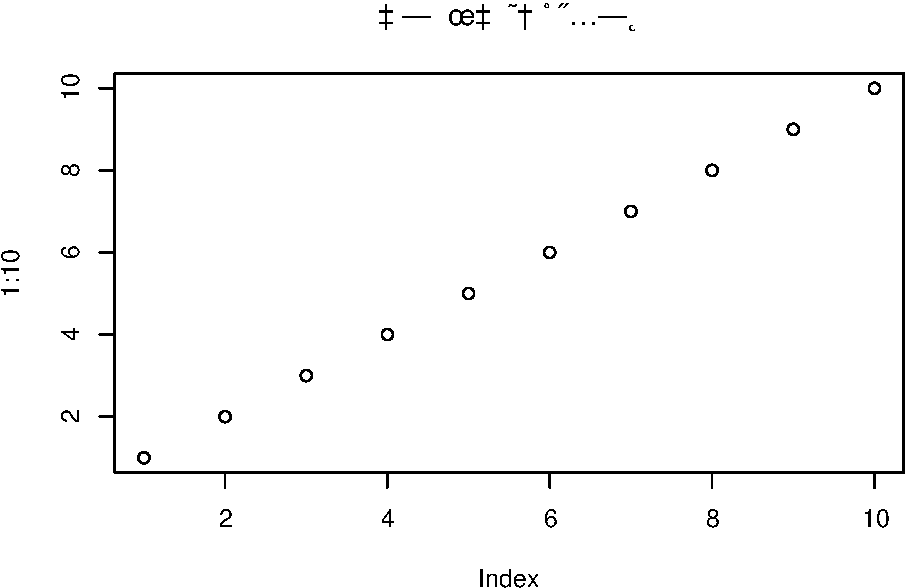
\includegraphics{0001-intro_files/figure-latex/u-w-f-ex01-1.pdf}
\caption{\label{fig:u-w-f-ex01}图形说明文字}
\end{figure}

引用如:参见图\ref{fig:u-w-f-ex01}。 引用中的\texttt{fig:}是必须的。

在通过LaTeX转换的PDF结果中, 这样图形是浮动的。

\hypertarget{causal}{%
\chapter{格兰格因果性}\label{causal}}

\hypertarget{causal-intro}{%
\section{介绍}\label{causal-intro}}

考虑两个时间序列之间的因果性。
这里的因果性指的是时间顺序上的关系,
如果\(X_{t-1}, X_{t-2}, \dots\)对\(Y_t\)有作用,
而\(Y_{t-1}, Y_{t-2}, \dots\)对\(X_t\)没有作用,
则称\(\{X_t \}\)是\(\{ Y_t \}\)的格兰格原因,
而\(\{ Y_t \}\)不是\(\{ X_t \}\)的格兰格原因。
如果\(X_{t-1}, X_{t-2}, \dots\)对\(Y_t\)有作用,
\(Y_{t-1}, Y_{t-2}, \dots\)对\(X_t\)也有作用,
则在没有进一步信息的情况下无法确定两个时间序列的因果性关系。

注意这种因果性与采样频率有关系,
在日数据或者月度数据中能发现的领先------滞后性质的因果关系,
到年度数据可能就以及混杂在以前变成同步的关系了。

\hypertarget{causal-def}{%
\section{格兰格因果性的定义}\label{causal-def}}

设\(\{ \xi_t \}\)为一个时间序列,
\(\{ \boldsymbol{\eta}_t \}\)为向量时间序列,
记
\[\begin{aligned}
\bar{\boldsymbol{\eta}}_t =& \{ \boldsymbol{\eta}_{t-1}, \boldsymbol{\eta}_{t-2}, \dots \} 
\end{aligned}\]

记
\(\text{Pred}(\xi_t | \bar{\boldsymbol{\eta}}_t)\)为基于
\(\boldsymbol{\eta}_{t-1}, \boldsymbol{\eta}_{t-2}, \dots\)
对\(\xi_t\)作的最小均方误差无偏预报,
其解为条件数学期望\(E(\xi_t | \boldsymbol{\eta}_{t-1}, \boldsymbol{\eta}_{t-2}, \dots)\),
在一定条件下可以等于\(\xi_t\)在\(\boldsymbol{\eta}_{t-1}, \boldsymbol{\eta}_{t-2}, \dots\)张成的线性Hilbert空间的投影
(比如,\((\xi_t, \boldsymbol{\eta}_t)\)为平稳正态多元时间序列),
即最优线性预测。
直观理解成基于过去的\(\{\boldsymbol{\eta}_{t-1}, \boldsymbol{\eta}_{t-2}, \dots \}\)的信息对当前的\(\xi_t\)作的最优预测。

令一步预测误差为
\[
  \varepsilon(\xi_t | \bar{\boldsymbol{\eta}}_t) 
  = \xi_t - \text{Pred}(\xi_t | \bar{\boldsymbol{\eta}}_t)
\]
令一步预测误差方差,或者均方误差,
为
\[
  \sigma^2(\xi_t | \bar{\boldsymbol{\eta}}_t)  
  = \text{Var}(\varepsilon_t(\xi_t | \bar{\boldsymbol{\eta}}_t) )
  = E \left[ \xi_t - \text{Pred}(\xi_t | \bar{\boldsymbol{\eta}}_t) \right]^2
\]

考虑两个时间序列\(\{ X_t \}\)和\(\{ Y_t \}\),
\(\{(X_t, Y_t) \}\)宽平稳或严平稳。

\begin{itemize}
\tightlist
\item
  如果
  \[
  \sigma^2(Y_t | \bar Y_t, \bar X_t) < \sigma^2(Y_t | \bar Y_t)
  \]
  则称\(\{ X_t \}\)是\(\{ Y_t \}\)的\textbf{格兰格原因},
  记作\(X_t \Rightarrow Y_t\)。
  这不排除\(\{ Y_t \}\)也可以是\(\{ X_t \}\)的格兰格原因。
\item
  如果\(X_t \Rightarrow Y_t\),而且\(Y_t \Rightarrow X_t\),
  则称互相有\textbf{反馈}关系,
  记作\(X_t \Leftrightarrow Y_t\)。
\item
  如果
  \[
  \sigma^2(Y_t | \bar Y_t, X_t, \bar X_t) < \sigma^2(Y_t | \bar Y_t, \bar X_t)
  \]
  即除了过去的信息,
  增加同时刻的\(X_t\)信息后对\(Y_t\)预测有改进,
  则称\(\{X_t \}\)对\(\{Y_t \}\)有瞬时因果性。
  这时\(\{Y_t \}\)对\(\{X_t \}\)也有瞬时因果性。
\item
  如果\(X_t \Rightarrow Y_t\),
  则存在最小的正整数\(m\),
  使得
  \[
  \sigma^2(Y_t | \bar Y_t, X_{t-m}, X_{t-m-1}, \dots) 
  < \sigma^2(Y_t | \bar Y_t, X_{t-m-1}, X_{t-m-2}, \dots) 
  \]
  称\(m\)为\textbf{因果性滞后值}(causality lag)。
  如果\(m>1\),
  这意味着在已有\(Y_{t-1}, Y_{t-2}, \dots\)和\(X_{t-m}, X_{t-m-1}, \dots\)的条件下,
  增加\(X_{t-1}\), \dots, \(X_{t-m+1}\)不能改进对\(Y_t\)的预测。
\end{itemize}

\begin{example}
\protect\hypertarget{exm:causal-exaxylag1}{}\label{exm:causal-exaxylag1}设\(\{ \varepsilon_t, \eta_t \}\)是相互独立的零均值白噪声列,
\(\text{Var}(\varepsilon_t)=1\),
\(\text{Var}(\eta_t)=1\),
考虑
\[\begin{aligned}
Y_t =& X_{t-1} + \varepsilon_t \\
X_t =& \eta_t + 0.5 \eta_{t-1}
\end{aligned}\]
\end{example}

用\(L(\cdot|\cdot)\)表示最优线性预测,则
\[\begin{aligned}
& L(Y_t | \bar Y_t, \bar X_t) \\
=& L(X_{t-1} | X_{t-1}, \dots, Y_{t-1}, \dots)
+ L(\varepsilon_t | \bar Y_t, \bar X_t) \\
=& X_{t-1} + 0 \\
=& X_{t-1} \\
\sigma(Y_t | \bar Y_t, \bar X_t) =&
\text{Var}(\varepsilon_t) = 1
\end{aligned}\]
而
\[
Y_t = \eta_{t-1} + 0.5\eta_{t-2} + \varepsilon_t
\]
有
\[\begin{aligned}
\gamma_Y(0) = 2.25,
\gamma_Y(1) = 0.5,
\gamma_Y(k) = 0, k \geq 2
\end{aligned}\]
所以\(\{Y_t \}\)是一个MA(1)序列,
设其方程为
\[
Y_t = \zeta_t + b \zeta_{t-1}, 
\zeta_t \sim \text{WN}(0, \sigma_\zeta^2)
\]
可以解出
\[\begin{aligned}
\rho_Y(1) =& \frac{\gamma_Y(1)}{\gamma_Y(0)} = \frac{2}{9} \\
b =& \frac{1 - \sqrt{1 - 4 \rho_Y^2(1)}}{2 \rho_Y(1)}
\approx 0.2344 \\
\sigma_\zeta^2 =& \frac{\gamma_Y(1)}{b} \approx 2.1328
\end{aligned}\]
于是
\[\begin{aligned}
\sigma(Y_t | \bar Y_t)
=& \sigma_\zeta^2 = 2.1328
\end{aligned}\]
所以
\[\begin{aligned}
\sigma(Y_t | \bar Y_t, \bar X_t) = 1
< 2.1328 = \sigma(Y_t | \bar Y_t)
\end{aligned}\]
即\(X_t\)是\(Y_t\)的格兰格原因。

反之,
\(X_t\)是MA(1)序列,
有
\[
\eta_t = \frac{1}{1 + 0.5 B} X_t
= \sum_{j=0}^\infty (-0.5)^j X_{t-j}
\]
其中\(B\)是推移算子(滞后算子)。
于是
\[\begin{aligned}
L(X_t | \bar X_t)
=& L(\eta_t | \bar X_t)
+ 0.5 L(\eta_{t-1} | \bar X_t) \\
=& 0.5 \sum_{j=0}^\infty (-0.5)^j X_{t-1-j} \\
=& - \sum_{j=1}^\infty (-0.5)^j X_{t-j} \\
\sigma(X_t | \bar X_t)
=& \text{Var}(X_t - L(X_t | \bar X_t)) \\
=& \text{Var}(\eta_t) = 1
\end{aligned}\]
而
\[\begin{aligned}
L(X_t | \bar X_t, \bar Y_t) 
=& L(\eta_t | \bar X_t, \bar Y_t)
+ 0.5 L(\eta_{t-1} | \bar X_t, \bar Y_t) \\
=& 0 +
0.5 L(\sum_{j=0}^\infty (-0.5)^j X_{t-1-j} | \bar X_t, \bar Y_t) \\
=& -\sum_{j=1}^\infty (-0.5)^j X_{t-j} \\
=& L(X_t | \bar X_t)
\end{aligned}\]
所以\(Y_t\)不是\(X_t\)的格兰格原因。

考虑瞬时因果性。
\[\begin{aligned}
L(Y_t | \bar X_t, \bar Y_t, X_t)
=& X_{t-1} + 0 (\text{注意}\varepsilon_t\text{与}\{X_s, \forall s\}\text{不相关} \\
=& L(Y_t | \bar X_t, \bar Y_t)
\end{aligned}\]
所以\(X_t\)不是\(Y_t\)的瞬时格兰格原因。

○○○○○

\begin{example}
\protect\hypertarget{exm:causal-exaxylag2}{}\label{exm:causal-exaxylag2}在例\ref{exm:causal-exaxylag1}中,如果模型改成
\[\begin{aligned}
Y_t =& X_{t} + \varepsilon_t \\
X_t =& \eta_t + 0.5 \eta_{t-1}
\end{aligned}\]
有怎样的结果?
\end{example}

这时
\[
Y_t = \varepsilon_t + \eta_t + 0.5 \eta_{t-1}
\]
仍有
\[\begin{aligned}
\gamma_Y(0) = 2.25,
\gamma_Y(1) = 0.5,
\gamma_Y(k) = 0, k \geq 2
\end{aligned}\]
所以\(Y_t\)还服从MA(1)模型
\[
Y_t = \zeta_t + b \zeta_{t-1},
b \approx 0.2344,
\sigma^2_\zeta \approx 2.1328
\]

\[\begin{aligned}
L(Y_t | \bar Y_t, \bar X_t)
=& L(X_t | \bar Y_t, \bar X_t) + 0 \\
=& L(\eta_t | \bar Y_t, \bar X_t)
+ 0.5 L(\eta_{t-1} | \bar Y_t, \bar X_t) \\
=& 0 + 0.5 L(\sum_{j=0}^\infty (-0.5)^j X_{t-1-j} | \bar Y_t, \bar X_t) \\
=& - \sum_{j=1}^\infty (-0.5)^j X_{t-j} \\
=& X_t - \eta_t \\
\sigma(Y_t | \bar Y_t, \bar X_t) 
=& \text{Var}(\varepsilon_t + \eta_t) = 2
\end{aligned}\]
而
\[
\sigma(Y_t | \bar Y_t)
= \sigma^2_\zeta \approx 2.1328
> \sigma(Y_t | \bar Y_t, \bar X_t) = 2
\]
所以\(X_t\)是\(Y_t\)的格兰格原因。

反之,
\[\begin{aligned}
L(X_t | \bar X_t, \bar Y_t)
=& - \sum_{j=1}^\infty (-0.5)^j X_{t-j} \\
=& L(X_t | \bar X_t)
\end{aligned}\]
所以\(Y_t\)不是\(X_t\)的格兰格原因。

考虑瞬时因果性。
\[\begin{aligned}
L(Y_t | \bar X_t, \bar Y_t, X_t)
=& X_{t} + 0 (\text{注意}\varepsilon_t\text{与}\{X_s, \forall s\}\text{不相关} \\
=& X_t \\
\sigma(Y_t | \bar X_t, \bar Y_t, X_t)
=& \text{Var}(\varepsilon) \\
=& 1 < 2 = \sigma(Y_t | \bar X_t, \bar Y_t)
\end{aligned}\]
所以\(X_t\)是\(Y_t\)的瞬时格兰格原因。

\[\begin{aligned}
[aaa]
\end{aligned}\]

\printbibliography

\end{document}
